\subsection{Implementation of \texttt{tmin(void)}}

To determine the minimum number representable by two's complement, we have to be aware of how two's complement works. Two's complement reserves the most significant bit as a sign bit --- i.e. if the bit is set, the number is negative, and otherwise it's nonnegative.

One might implement signed integers intuitively in a way where positive and negative number pairs share all bits other than the sign bit (i.e. 3 and -3 would be represented as \code{011} and \code{111}, respectively). However, this is makes addition and overflow difficult to implement.

Two's complement is a way to make addition and subtraction easier to handle. To obtain that, the negative half of the numbers are represented in ``reverse'' (see \autoref{fig:twos-complement}). That is, for 4-bit integers, instead of having \code{1000} represent (negative) 0, we make it represent -8. Likewise, instead of having \code{1111} represent -7, we make it represent -1. This means that when you add 1 to the maximum number, you get the minimum number by nature of the representation.

\begin{figure}[H]
  \centering
  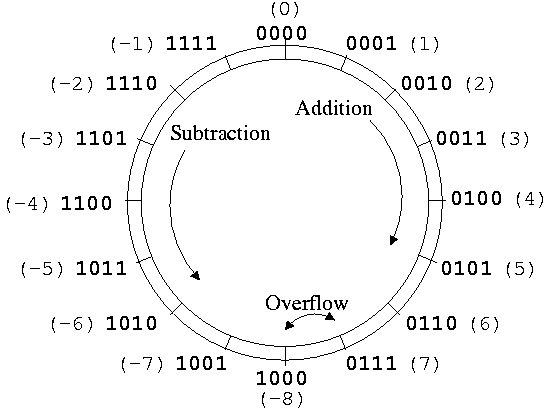
\includegraphics[width=0.7\textwidth]{figures/twos-complement.png}
  \caption[nothing]{An illustration of how integers are represented using two's complement~\cite{twoscomplement}.}
  \label{fig:twos-complement}
\end{figure}

With this in mind, we know that, by two's complement, the smallest number starts with a 1 followed by 0s only. Thus we can obtain the smallest number representable by two's complement by shifting a 1 to the most significant bit's position.

When you shift to the left with \code{<<}, all of the ``new'' bits on the right side are set to 0. For example \code{1011 << 2} becomes \code{1100} (assuming there is only space for 4 bits).

My complete implementation of \code{tmin(void)} is as follows:

\begin{minted}{c}
int tmin(void) {
  return 1 << 31;
}
\end{minted}

Because we are working with 32-bit numbers, shifting a 1 to the left by 31 bits will yield a single 1 in the most significant bit's position and nothing but 0s elsewhere. In decimal, this number is -2147483648.
